\newpage
\section{Reflexion der Ergebnisse} \label{fazit}
Die Ergebnisse die sich aus den Analysen ergeben sind für die aufgewendete Zeit anschaulich und repräsentativ. Diese können aber durch weitere Betrachtungen, in Hinblick auf einen Mobilitätsindex, weiter gesteigert werden.
% Die gezeigten Ansätze können sowohl für eine deskriptive und dynamische Repräsentation genutzt werden aber auch für professionelle Städteplaner oder gar Entscheider in der öffentlichen Hand. 
% Das Portal bzw. die Berlin-Mobility.web.app ermöglicht jedem auf Informationen zuzugreifen und diese anschaulich zu präsentieren.

\subsection{Lessons Learned}
Aus den Ergebnissen ist klar erkennbar, dass die innerstädtischen Wohngebiete bereits gut angebunden sind. Das wurde in Kapitel \ref{projektergebnisse} anschaulich sowohl mit den Isochronen aber auch mit der Verteilung der Verkehrsmittel gezeigt. 
Bei der Anbindung von Industrie- und Handel gibt es Handlungsbedarf. Die Verzahnung des bereits bestehenden ÖPNV Angebotes muss effizienter und effektiver gestaltet werden.

Des Weiteren ist zur besseren Vernetzung unterschiedlicher Verkehrsmittel die Entwicklung und der Ausbau von Mirkomobilitätskonzepten (bspw. Jelbi) zu prüfen und zu fördern.
Denn nur mit einem breiten diversen Angebot kann die nötige Tiefe und nachhaltige Wende in Berlin eingeleitet werden.​​

Der Plan zum Ausbau der Straßenbahn in die nord-westlichen Bezirke hat großes Potenzial. Der Senat hat ähnliche Bedarfe im Süden identifiziert, dieser Bedarf kann ausgehend von der Analyse bestätigt werden.
Wie bereits erwähnt kann damit ein breites Angebot genutzt werden. Dies wiederum führt zu einer Entlastungen in den entsprechenden Verkehrsmitteln oder Angeboten der Mobilität.

Die Außenbezirke sind häufig stark auf einzelne Linien angewiesen und eine Abhängigkeit entsteht. Die Vernetzung unterschiedlicher Verkehrsmittel ist einer der Schlüssel zur Gestaltung der Verkehrswende in Berlin. ​

\todo[inline]{MEHR !!! \% mehr Inhalt zur Anreicherung}

\subsection{Limitierungen}
\subsubsection{Datenverfügbarkeit und Qualität}
Es konnten nicht alle Dimensionen betrachtet werden aufgrund der fehlenden Verfügbarkeit von Daten. Als Beispiel kann die Zahl der Beschäftigten in Gewerbe-, Handels- und Industriegebieten genannt werden. Diese sind nicht automatisiert erfasst bzw. zu ermitteln​ sowie deren aktualität konnte nicht gewährleistet werden.
Denn die Dichte bestimmt maßgeblich das zu erwartende Volumen an möglichen Fahrgästen oder Nutzern in den entsprechenden Regionen. Denn großflächige Gewerbe oder Industriegebiete können durch einen hohen automatisierungsgrad sehr gering ausfallen.

Eine weitere Limitierung gibt es in der Quantität der Daten zu den tatsächlichen Geschwindigkeiten des Autoverkehrs. Diese liegen nicht für alle Straßenabschnitte/-segmente vor​. Grund dafür ist, dass die Messungen durch einen privaten Fahrdienst, Uber, aufgenommen wurden. Demzufolge konnten nicht alle Straßen mit Metriken ausgestattet werden. 
Diese fehlenden Metriken bzw. Segmente würden eine ganzheitliche Betrachtung des Straßenverkehrs ermöglichen und helfen dabei vollständiges Bild zeichnen.

Zuverlässige Daten zur Auslastung des ÖPNV sind nicht verfügbar​. Diese Daten hätten Aussagen dazu liefern können, wann die verschiedenen Medien des ÖPNV wie stark ausgenutzt sind.

Gründsätzlich wurden Wasserflächen nicht vollständig betrachtet. Darunter zählen Enzitäten wie Hausboote, gewerbliche Flächen und Verkehrsmittel auf dem Wasser.

\todo[inline]{MEHR !!! \% mehr Inhalt zur Anreicherung}

\subsubsection{Komplexität der Analyse}
Die Dimension der Taktung des ÖPNV wird in der Analyse nicht berücksichtigt​.

Es wird kein „Penalty“ zur Nutzung des Autos eingerechnet aber auch nicht für die ÖPNV eingerechnet​. Dieser Umstand sollte in kommenden Analysen korrigiert werden.
Hintergrund ist, das für die Nutzung im innerstädtischen Bereich eine Parkplatzsuche oder das erreichen des Verkehrsmittels mit eingrechnet werden müsste.
Deshalb wurde sich in dem ersten Wurf dafür entschieden, keine Bestrafung für irgendeine Form der Fortbewegung einzurechnen. 
Beim ÖPNV wären es zum Beispiel die Umsteigezeiten oder Umsteige wege selbst auf Haltestellen etc.. 
Genauso auch das tatsächliche Erreichen des Bahnsteiges wurde nicht betrachetet. Demzufolge wurde sich bei jeder Analyse für kein „Penalty“ entschieden.
Auch die die Barrierefreiheit von Haltestellen/Stationen wird nicht berücksichtigt​ und es findet in dieser Dimension keine Analyse statt.

Aktuell werden ausschließlich 15 Minuten Isochrone analysiert​. Aufgrund der nötigen Ressourcen musste sich für eine Ausprägung entschieden werden.
Es wurde sich für 15 Minuten entschieden, weil es nicht zu viel für PKWs ist aber auch nicht zu wenig für die anderen Verkehrsmittel.

\todo[inline]{MEHR !!! \% mehr Inhalt zur Anreicherung}

\subsubsection{Blick von außen}
Ein neutraler Blick auf die Verkehrsdaten hilft dabei Voreingenommenheit zu vermeiden und Herausforderungen aus einem neuen Blickwinkel zu betrachten.​
Analyse-Ergebnisse zeigen Schwerpunkte, die eine besonders eingeschränkte Erreichbarkeit aufweisen. Für das Validieren der Lösungsvorschläge und für die Planung neuer Verkehrswege benötigt es jedoch spezifisches Domänenwissen​

\todo[inline]{MEHR !!! \% mehr Inhalt zur Anreicherung}

\subsection{Future Work / Folgeprojekte}

\subsubsection{Anreicherung der Analyse}
Anreicherung der Analyse durch Berücksichtigung weiterer Faktoren wie Taktung, Verkehrssicherheit, Lärmbelästigung und Klimaschutz wären sinnvoll.
Auch das Nutzen von „Bestrafungen“ oder „Penaltys“ als Komplexitätssteigerung ist denkbar und nötig. Dies würde im Bereich der Verkehrsmittel zu einer Glättung führen aber auch ggf. zu einer positiven Einflussnahme.
Darunter ist zum Beispiel das Tanken von privaten PKWs gemeint. Bei der Nutzung kommt eine gewisse Abhängigkeit bzw. Zusatzbedingung in die Gleichung.
Auch das nicht ganz unabhängige abstellen von Verkehrsmitteln von Sharingdiensten kann damit entsprechend beeinflusst werden und die Realität näher abbilden.

\todo[inline]{MEHR !!! \% mehr Inhalt zur Anreicherung}

\subsubsection{Finalisierung des Dashboards}
Zur Verfügungstellung eines Modus zur individuellen Verkehrsanalyse welcher Bürger*innen zur Verfügung gestellt werden kann, um die Bürgerkommunikation zu verbessern.
Hier können auch aktuelle Projekte die Betrachtung ergänzen. Vielleicht könnte auch ein Votingsystem eingeführt werden, welches das Gefühl der Teilhabe steigert.
Das Dashboard kann und soll entsprechend weiter ausgebaut. 

\todo[inline]{MEHR !!! \% mehr Inhalt zur Anreicherung}

\subsubsection{Entwicklung eines Planungstools}
Einarbeitung möglicher bzw. geplanter Streckenverläufe um Potenzial von Infrastrukturvorhaben unkompliziert und visuell evaluieren zu können.

\todo[inline]{MEHR !!! \% mehr Inhalt zur Anreicherung}

\subsubsection{Blick von außen}
Die Projektgruppe hat während des Verlaufs immer mehr an Erfahrungen in der Domäne der innerstädtischen Mobilität gewonnen. Um hier eine breitere und tiefere Weiterentwicklung anzustreben, muss der Blick von außen gebrochen werden.
Für eine Weiterentwicklung sollten weitere Experten wie Städteplaner oder Stakeholder aus der öffentliches Hand frühzeitig mit eingebunden werden.

Mit mehr Ressourcen könnte auch die Ausweitung oder Reduzierung der Domäne betrachtet werden. Darunter zählt die Urbanisierung sowie die Suburbanisierung.
Ersteres ist die allgemeinbekannte Landflucht und letzteres ist die Stadflucht. Beide beschreiben die Veränderung von Regionen oder Domänen. 
Diese Einflussnahme sollte mit Experten zusammen weiter betrachtet werden und ggf. Maßnahmen für eine Stabilisierung bzw. für ein sinnvolles Gleichgewicht in der Urbanisierung oder Suburbanisierung gefunden werden.

Auch die Sozioökonomischen und ökologischen Perpektiven sollten vertieft werden. 
%Letzteres kann den Forstämtern dabei helfen Wild und deren Pupolation besser zu Steuern aber auch das schaffen neuer Räume für gefärdete Arten zeitig auszuschreiben.
Den nicht trennscharf eingeführten Begriff der Sozioökonomie könnte unteranderem die Entwicklung eines fortlaufenden Mobilitätsindex, um Veränderungen in der Anbindungsqualität feststellen zu können und zur Identifizierung weitere weitere Maßnahmen.

\todo[inline]{AUFFÜHREN UND QUELLEN NUTZEN !!! \% aufzeigen das keine Trennschärfe existiert und ggf. ein oder zwei Aussagen hinzufügen}

Hierbei könnten sowohl Ökologische aber auch Ökonomische Aspekte verstärkt gewichtet werden. %Damit könnten sich die Bewohner oder Nutzer einer Domäne vielleicht besser identifizieren.
Auch der Vergleich mit anderen Städten oder Landkreisen könnte hier wichtig sein. Es wurde nur der Ballungsraum Berlin betrachtet und das Umland wurde nicht betrachtet. Das schmälert das Gewicht der Pendler. Alles in Allem muss der Mobilitätsindex Formalisiert werden. 

Gewichte die in einem Mobilitätsindex ein Rolle spielen könnten unter anderm Anteil an Miet- und Eigentumswohnungen sowie die Einwohner-, 
Gewerbe oder Industriedichte. Auch die durchschnittliche Geschwindigkeit aller möglichen Verkehrsmittel, 
die ÖPNV Streckendichte (verschiedene Medien summieren), die ÖPNV Haltestellendichte oder die Straßendichte mit Fahrradwegen und PKW/LKW Wegen.
Als negativbeispiel kann der formalisierte Mobilitätsindex genannt werden.



%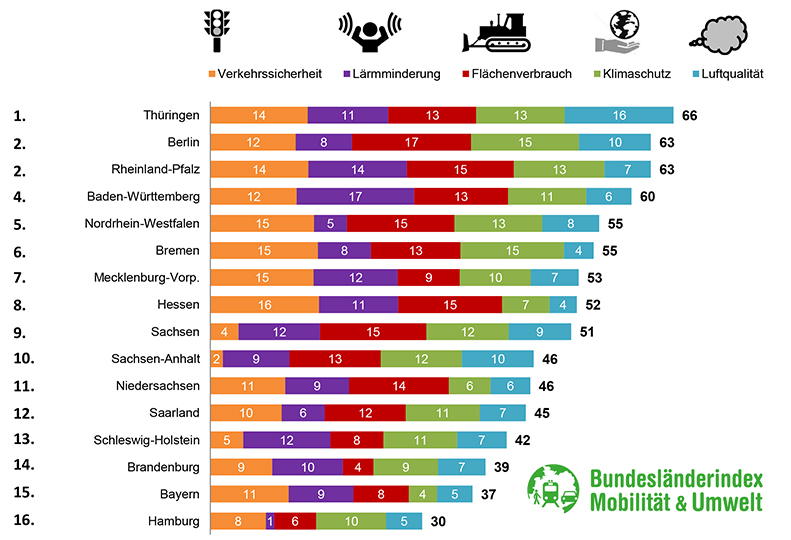
\includegraphics{​​​​../abbildungen/Mob-Index.jpg}
%\includegraphics[width=11cm]{abbildungen/mob-index} \\
\img{mob-index}{width=14cm}{Mobilitätsindex}
%\img{​​​​mob-index}​{​​​​width=11cm}​​​​{​​​​Mobilitätsindex}​​​​

\todo[inline]{QUELLE - EINBINDEN UND LINK \% https://www.allianz-pro-schiene.de/wp-content/uploads/2015/08/blimu-100.jpg}

"Fünf Themen fließen in das Gesamtergebnis ein: Verkehrssicherheit, Lärmminderung, Flächenverbrauch, Klimaschutz und Luftqualität."

\todo[inline]{PRÄZISIEREN !!! \% weiter ausführen und genauen Vergleich mit QUellen angeben}

Alle fünf Themen sind wichtig aber können keine Aussage zur Mobilität geben. Alleine das fehlen, des bereits erwähnten Gewichtes, der Durschnittsgeschwindigkeit lässt an der Gültigkeit und Aussagekraft eines Mobilitätsindexes zweifeln.
Deshalb sollte viel Kraft in die ausgewogene und gut gewichtete Gestaltung eines formalen allgemeingültigen Mobilitätsindexes gesetzt werden.

Auch die genutzten Quellen sollten nicht statisch sein sondern wie in dem Projekt dynamsich sein. Das ermöglicht ein ständig sich anpassendes Bild. Der Index lebt wie die Stadt bzw. der Raum selbst der bewertet werden soll.
